\documentclass{standalone}

\usepackage{amsmath}
\usepackage{tikz}
\usetikzlibrary{circuits.ee.IEC}
\usepackage{placeins}

\begin{document}
	
	
	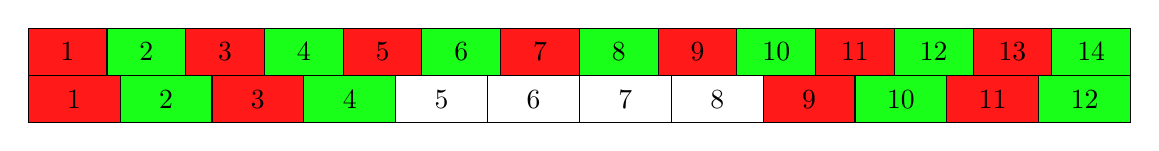
\begin{tikzpicture}[
		point/.style={circle,draw,minimum size=#1},
		point/.default=0pt]
		
		
		%rotor
		\foreach \i/\farbe [evaluate=\i as \x using int(1*\i)] in {1/red!90,2/green!90,3/red!90,4/green!90,5/red!90,6/green!90,7/red!90,8/green!90,9/red!90,10/green!90,11/red!90,12/green!90,13/red!90,14/green!90} 
		{
			\draw[fill=\farbe] (\x-1,0) rectangle (\x,0.6); 
			\node at (\x-0.5,0.3) {\i};
		}
			
		
		%stator
		\foreach \i/\farbe  [evaluate=\i as \x using (14/12*\i)] in {1/red!90,2/green!90,3/red!90,4/green!90,5/white!90,6/white!90,7/white!90,8/white!90,9/red!90,10/green!90,11/red!90,12/green!90} 
		{
			\draw[fill=\farbe] (\x-14/12,-0.6) rectangle (\x,0);
			\node at (\x-14/24,-0.3) {\i};
		}
		
			
	\end{tikzpicture}


\end{document}